\documentclass{article}
\usepackage{fancyhdr}
\usepackage{amsmath,amssymb}
\usepackage{geometry}
\usepackage{datetime}
\usepackage{enumerate}
\usepackage{graphicx}

%Insert page formatting here
\hoffset = -.5in
\voffset = -0.375in
\textwidth = 7in
\textheight = 8in
\headheight = 24pt

\pagestyle{fancy}

\rhead{Peter Olson\\Student ID: $441666$}
\lhead{Math 3200\\Homework 10}
\chead{\today}
\cfoot{}

%\addtolength{\headwidth}{\marginparsep}
%\addtolength{\headwidth}{\marginparwidth}

%\renewcommand{\labelitemi}{$\diamond$}
\renewcommand{\implies}{\rightarrow}
\newcommand{\widespace}{\qquad \qquad \;}
\newcommand{\tret}{\\ \hline}
\newcommand{\fh}{\tfrac{1}{2}}
\newcommand{\deriv}[2]{\frac{d #1}{d #2}}
\newcommand{\pderiv}[2]{\frac{\delta #1}{\delta #2}}
\newcommand{\vr}{\vec{r}}
\newcommand{\at}{\text{ at }}
\newcommand{\var}{\text{Var}}
\newcommand{\cov}{\text{Cov}}

\begin{document}

\section*{Exercise 10.5 + (d) + (e)}

\begin{enumerate}[\quad(a)]
	\item Make a scatter plot for the length of the jump by year. Does the relationship appear to be approximately linear?\\
	\begin{center}
		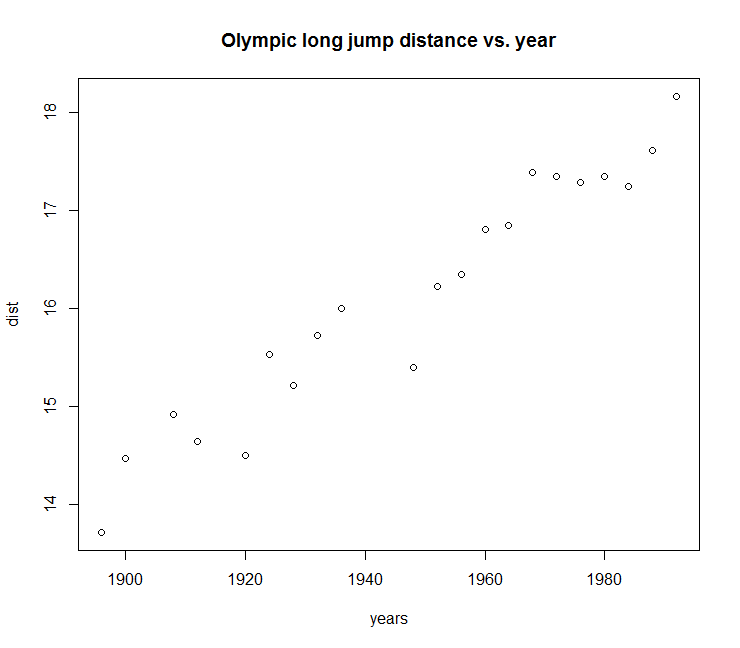
\includegraphics[width=3.5in]{Q31.png}
	\end{center}
	The relationship appears approximately linear.
	\item Fit a least squares regression line.\\
	\begin{center}
		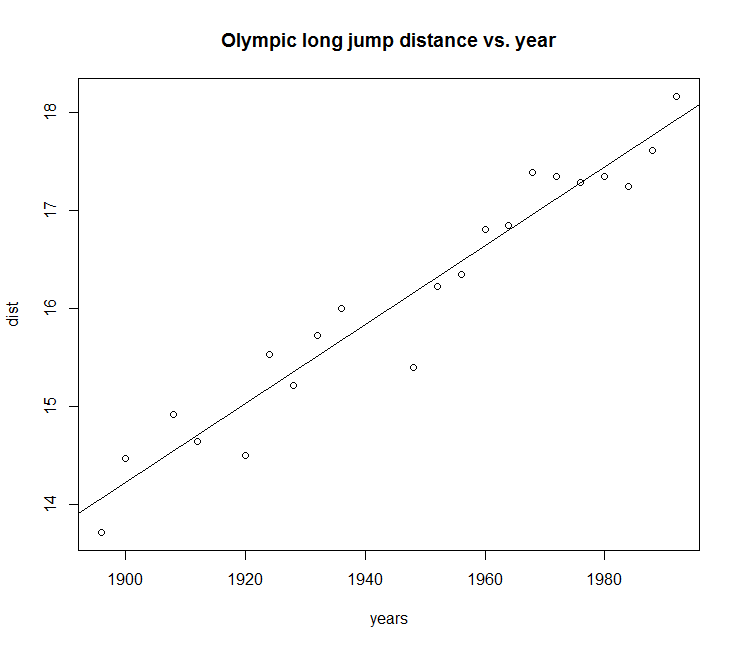
\includegraphics[width=3.5in]{Q32.png}
	\end{center}
	\item Calculate the mean squares error estimate of $\sigma$.

	$\sigma =$ \texttt{0.3227}
	\item What is the proportion of the variability in ``Winning Distance'' that is accounted for (or explained by) ``Year''?

	The $r^2$ value from the fit is \texttt{0.9371}
	\item Calculate the sample correlation coefficient and a 95\% confidence interval for the correlation coefficient. Is the correlation between ``Winning Distance'' and ``Year'' significantly positive?

	Given that the correlation coefficient is \texttt{0.9680191}, it's sufficient to say that the data is significatly correlated.
\end{enumerate}

\section*{Exercise 10.9}

\begin{enumerate}[\quad(a)]
	\item Is there a significant linear trend in the jump distance? Test at $\alpha = 0.05$.

	Given that $t_{21-2, 0.05/2} = t_{19, 0.025} = 2.093$, and $|t| = 16.81901$, we can safely reject $H_0: \beta = 0$ and accept that there is a linear correlation between the distanced jumped and the year.

	\item Calculate a 95\% PI for the winning jump in 2004. Do you think this prediction is reliable? Why or why not? Would a 95\% CI for the winning jumpin 2004 have a meaningful interpretation? Explain.

	The 95\% prediction interval for the longest long jump in 2004 is $[ 17.66201, 19.15632 ]$. I don't think this prediction is reliable, or meaningful, as extrapolating the results of a simple linear model beyond the range of a data set without a very, very good reason to do so seems too risky for me to put much stock in. Plus, the prediction only anticipates that the longest long jump at the Olympics is going to be at least equivalent to the longest jump from 1980, almost 24 years ago, and that the maximum is just a freakish increase in length. The only meaningful interpretation of the prediction is that we can expect with high certainty that the longest jump is going to be close to what it was last year.
\end{enumerate}

\section*{R Output}
\begin{verbatim}
> # echo out the mse
> fit_mse
[1] 1.406501

> # echo out the r^2 value
> summary(fit)[['r.squared']]
[1] 0.9370609

> # calculate the cor
> cor(dist, years)
[1] 0.9680191

> # echo out t's Student-t test
> t
[1] 16.81901

> # echo out the length of the data set
> length(years)
[1] 21

> predict(fit, newjump, interval="predict")
       fit      lwr      upr
1 18.40916 17.66201 19.15632
\end{verbatim}

\section*{R Code}
\begin{verbatim}
# Prepare data
years <- c(
  1896, 1900, 1908, 1912, 
  1920, 1924, 1928, 1932, 
  1936, 1948, 1952, 1956, 
  1960, 1964, 1968, 1972, 
  1976, 1980, 1984, 1988, 
  1992
)

dist <- c(
  13.71, 14.47, 14.92, 14.64,
  14.50, 15.53, 15.21, 15.72,
  16.00, 15.40, 16.22, 16.35,
  16.81, 16.85, 17.39, 17.35,
  17.29, 17.35, 17.25, 17.61, 
  18.17
)

#
# 10.5
#

# a
plot(years, dist, main = "Olympic long jump distance vs. year")

# b
fit <- lm(dist~years)
# Add line to plot
abline(fit)

# c
sqrt(sum(resid(fit)^2) / (length(years) - 2))

# d
# echo out the r^2 value
summary(fit)[['r.squared']]

# e
# calculate the cor
cor(dist, years)
#
# 10.9
#

# a
t <- coef(summary(fit))[2, "Estimate"] / coef(summary(fit))[2, "Std. Error"]
# echo out t's Student-t test
t
# echo out the length of the data set
length(years)

# b
# create dataframe for prediction
newjump = data.frame(years=2004)
# echo out prediction
predict(fit, newjump, level = 0.05, interval="predict")

\end{verbatim}

\end{document}